% ============================================================
% 主控文件：只负责整合，不写具体内容
% 编译器请选择 XeLaTeX
% ============================================================

\documentclass[12pt,a4paper]{ctexart}
\usepackage{xeCJK}

% ---------- 导入导言区 ----------
% ============================================================
% 导言区：所有宏包、页面设置、样式命令
% ============================================================

% ---------- 页面设置 ----------
\usepackage{geometry}
\geometry{left=2.5cm,right=2.5cm,top=2.5cm,bottom=2.5cm}

% ---------- 数学与符号 ----------
\usepackage{amsmath, amssymb, amsfonts}
\usepackage{bm}          % 加粗数学符号
\usepackage{cases}       % 分段函数环境

% ---------- 表格与图形 ----------
\usepackage{float}
\usepackage{booktabs}    % 三线表
\usepackage{graphicx}    % 插图
\usepackage{caption}     % 图注、表注
\usepackage{subcaption}  % 子图
\usepackage{array}       % 增强表格列
\usepackage{multirow}    % 合并单元格
\usepackage{longtable}   % 长表格

% ---------- 代码与列表 ----------
\usepackage{listings}    % 代码插入
\usepackage{xcolor}      % 颜色

\usepackage{adjustbox} % 
\lstset{
    basicstyle=\ttfamily\small,
    breaklines=true,
    frame=single,
    numbers=left,
    numberstyle=\tiny,
    keywordstyle=\color{blue},
    commentstyle=\color{green!60!black},
    stringstyle=\color{red},
    tabsize=4
}

% ---------- 参考文献与超链接 ----------
\usepackage{hyperref}
\hypersetup{
    colorlinks=true,
    linkcolor=black,
    citecolor=black,
    urlcolor=black
}
\usepackage[numbers]{natbib}

% ---------- 其他工具 ----------
\usepackage{indentfirst} % 首段缩进
\usepackage{fancyhdr}    % 页眉页脚（可选）
\usepackage{enumitem}    % 列表定制
\usepackage{float}       % 强制图片位置 [H]


% ---------- 标题信息 ----------
\title{\textbf{板凳龙沿螺线运动的建模分析}}  % 替换成你的题目

\begin{document}
\pagestyle{empty}
% ---------- 生成标题 ----------
\maketitle

% ---------- 摘要 ----------
% ============================================================
% 摘要与关键词
% ============================================================

\begin{abstract}
\noindent 针对问题一，，首先根据舞龙队沿等距螺线盘入的运动特征，建立阿基米德螺线运动模型，并利用弧长关系确定任意时刻龙头前把手的极角。对于非线性方程难以直接求得解析解的问题，采用二分法进行数值求解。在此基础上，以相邻把手间的固定距离为几何约束，利用余弦定理建立相邻把手极角差的非线性方程，并通过二分法求取满足盘入方向的最小正根，逐节递推得到其余把手的极角及平面坐标，从而实现任意时刻舞龙队各把手位置的确定。此后，再通过求导的方式实现各点速度的求解。
\end{abstract}

\vspace{0.5cm}
\noindent \textbf{关键词：} 关键词一，关键词二，关键词三 





% ---------- 正文各章节 ----------
% ============================================================
% 第1章 问题背景与重述
% ============================================================

\section{问题重述}

\subsection{问题的背景}
板凳龙是浙闽地区传统民俗活动，由数十至上百条板凳首尾相连，形成蜿蜒长龙。舞龙时，龙头率先沿螺线盘入，龙身和龙尾依次跟随，整体呈圆盘状。表演中，在能自如盘入和盘出的前提下，所需场地面积越小、行进速度越快，观赏性越高。本题针对由223节板凳组成的舞龙队，龙头板长341 cm，龙身和龙尾板长220 cm，板宽30 cm，各节设有两个孔，孔径5.5 cm，孔中心距板头27.5 cm，相邻板凳通过把手连接。需建立数学模型，研究沿等距螺线运动时各把手的位置与速度、碰撞终止时刻、调头空间及最小螺距、S形调头路径优化以及最大行进速度等问题，为舞龙表演的规划与控制提供理论依据。

\subsection{问题的提出}
某板凳龙由223节板凳组成，其中第1节为龙头，其后221节为龙身，最后1节为龙尾。龙头板长为341 cm，龙身和龙尾板长均为220 cm，板宽均为30 cm。每节板凳上开有两个圆孔，孔径5.5 cm，孔中心距最近的板头27.5 cm，相邻板凳通过把手穿过圆孔连接。舞龙队沿螺距为55 cm的等距螺线顺时针盘入，各把手中心均位于螺线上，龙头前把手行进速度恒为1 m/s，初始时龙头位于螺线第16圈A点。

\textbf{问题1：}建立舞龙队沿给定螺线运动的数学模型，给出从初始时刻到300 s内每秒整个舞龙队各把手中心（包括龙头、龙身和龙尾各前把手及龙尾后把手）的位置和速度，将结果保存至文件result1.xlsx中；并在论文中列出0 s、60 s、120 s、180 s、240 s、300 s时龙头前把手、龙头后第1、51、101、151、201节龙身前把手和龙尾后把手的位置和速度。

\textbf{问题2：}在问题1设定的盘入螺线基础上，确定因相邻板凳发生碰撞而不能再继续盘入的终止时刻，并给出此时上述指定把手的位置和速度，将结果保存至result2.xlsx。

\textbf{问题3：}从盘入到盘出需要调头，调头空间为以螺线中心为圆心、直径为9 m的圆形区域。确定最小螺距，使得龙头前把手能够沿相应的螺线盘入至该调头空间边界，即恰好与调头区域相切。

\textbf{问题4：}盘入螺距为1.7 m，盘出螺线与盘入螺线关于螺线中心呈中心对称，调头路径为由两段圆弧相切连接而成的S形曲线（前一段圆弧半径是后一段的2倍），且与盘入、盘出螺线均相切。研究能否调整两段圆弧（仍保持相切）使调头曲线更短。以调头开始时刻为零时刻，给出从-100 s到100 s内每秒舞龙队的位置和速度，将结果保存至result4.xlsx，并在论文中列出-100 s、-50 s、0.5 s、50 s、100 s时指定把手的位置和速度。

\textbf{问题5：}在问题4设定的完整路径（盘入—调头—盘出）下，龙头行进速度保持不变，确定龙头的最大行进速度，使得舞龙队各把手的速度均不超过2 m/s。

      % 问题背景与重述
% ============================================================
% 第2章 问题分析
% ============================================================

\section{问题分析}

\subsection{问题一分析}
针对问题一，板凳龙沿螺距为$55~\text{cm}$的等距螺线盘入，各把手中心均位于螺线上，需在龙头前把手恒速$1~\text{m/s}$条件下确定$0\sim300~\text{s}$内所有把手的位置和速度。由于所有把手均在同一螺线上，不宜将各把手坐标作为独立变量，而应以\textbf{螺线极角$\theta$}为位置参量进行\textbf{参数化}建模。首先，将龙头运动转化为弧长参数化问题，利用\textbf{阿基米德螺线弧长微分公式}建立\textbf{弧长}函数，由龙头速度恒为$1~\text{m/s}$得$\boxed{S(\theta_1(t))=t}$，通过求解该一元方程得到\textbf{龙头极角}$\theta_1(t)$，从而确定任意时刻龙头前把手对应的螺线参数及其位置。随后，利用相邻把手距离固定的\textbf{几何约束}$\boxed{\left| P(\theta_{i+1})-P(\theta_i) \right| = L_i}$，构造关于$\theta_{i+1}$的非线性方程，并利用\textbf{余弦定理$+$二分检验搜索求解}，之后逐节递推求得所有把手的极角。最后，对龙头恒速条件直接求导得到\textbf{龙头角速度}，其余把手速度则通过先对$x$,$y$方向上分量分别求解，再合成为总速度的方式计算。我们利用“弧长参数化+逐节递推+二分法+隐式求导”的策略，使多体运动问题分解为一系列一维问题，有效降低了计算复杂度。



\subsection{问题二分析}
针对问题二，我们需要在已知板凳龙所有把手的运动状态的条件下，去判断舞龙队在盘入过程中何时首次发生板凳碰撞。已知每节板凳具有一定的长度和宽度，因此，本文首先将每节板凳抽象为以相邻把手连线为中心线、长度为$341cm$或$220cm$，宽度为$30cm$的矩形。其次，对于任意时刻$t$，利用问题一中的递推模型计算全部把手位置；随后由相邻把手确定各节板凳的位置和姿态，并利用$SAT$矩形碰撞判定方法判断任意两节非相邻板凳是否发生重叠。最后，利用和问题一中类似的基于二分法的时间搜索，求解首次检测碰撞时刻，将该时刻定义为舞龙队的临界盘入时刻$t^*$。

\subsection{问题三分析}
对第三个问题的扩展性和复杂点进行分析。        % 问题分析
% ============================================================
% 第3章 模型假设与符号约定
% ============================================================

\section{模型假设}
\begin{enumerate}[leftmargin=2em]
    \item 
    \item 
    \item 
\end{enumerate}

\section{符号说明}

\begin{table}[htbp]
\centering
\caption{主要符号说明}
\begin{tabular}{c|c|c}
\toprule
符号 & 含义 & 单位 \\
\midrule
$d$ & 外延层厚度 & $\mu$m \\
$\tilde{\nu}$ & 波数 & cm$^{-1}$ \\
$n$ & 复折射率 & --- \\
\bottomrule
\end{tabular}
\end{table}     % 模型假设与符号
% ============================================================
% 第4章 问题1 模型建立与求解
% ============================================================

\section{模型建立与求解——问题1}

\begin{figure}[htbp]
    \centering
    \begin{adjustbox}{center}
        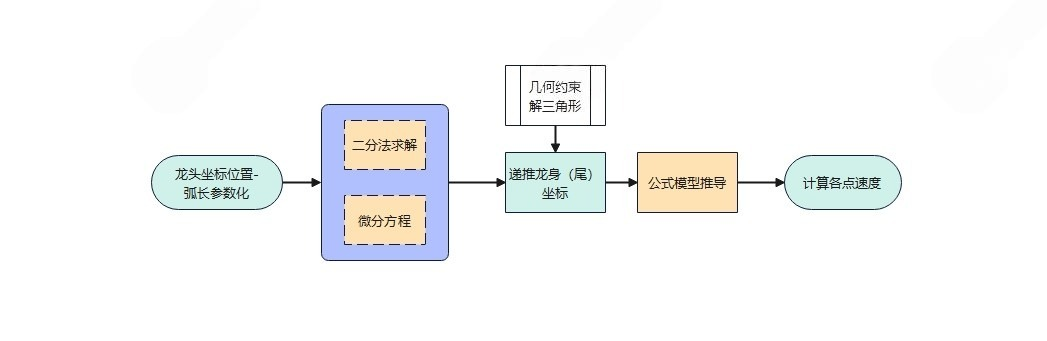
\includegraphics[width=1.3\columnwidth]{images/问题一流程图.jpeg}
    \end{adjustbox}
    \caption{问题一流程图}
    \label{fig:first}
\end{figure}

\subsection{弧长参数化和弧长函数}

由阿基米德螺线描述：
\begin{equation}
    r(\theta) = a + b\theta
\end{equation}
其中 $\theta$ 为极角，$r$ 为极径。螺距 $p=0.55\,\mathrm{m}$ 对应极角每增加 $2\pi$ 时极径的增量，同时由题图，$a$=0，故有：
\begin{equation}
    r(\theta) = b\theta
\end{equation}

\begin{equation}
b = \frac{p}{2\pi} = \frac{0.55}{2\pi}
\end{equation}
由此，螺线上任意点的直角坐标即为：
\begin{equation}
P(\theta) = (r(\theta)\cos\theta,\, r(\theta)\sin\theta)
\end{equation}
为描述龙头沿螺线的运动，需建立极角变化与弧长变化之间的关系。由上述参数方程求导，结合螺线极坐标表达式可得：
\begin{equation}
\frac{ds}{d\theta} = \sqrt{r^2 + b^2} = \sqrt{(a+b\theta)^2 + b^2}
\end{equation}
已知龙头速度恒定为$1~\text{m/s}$，经计算：
\begin{equation}
s(\theta) = \int_{\theta_0}^{\theta} \sqrt{(a+bu)^2 + b^2}\, du
\end{equation}
于是对于每一个时刻$t$,求解：
\begin{equation}
s(\theta(t)) = s(\theta_0) + t
\end{equation}
这实际上是一个一维非线性方程求根问题。



\subsection{龙头位置求解}
对于某一个具体时刻 $t = t_k$，我们要求：
\begin{equation}
f(\theta) = S(\theta) - t_k = 0
\end{equation}
由于 $S(\theta)$ 在龙头运动范围内具有单调性，因此上述方程具有唯一解。对于给定时刻 $t$，采用二分法求解 $\theta_1(t)$。
具体而言，首先确定包含根的区间 $[\theta_L,\theta_R]$，使得
\begin{equation}
f(\theta_L)f(\theta_R)<0,
\end{equation}
其中
\begin{equation}
f(\theta)=S(\theta)-t.
\end{equation}

随后取区间中点
\begin{equation}
\theta_M=\frac{\theta_L+\theta_R}{2},
\end{equation}
根据 $f(\theta_M)$ 的符号判断根所在区间，并不断缩小搜索区间。当满足
\begin{equation}
|\theta_R-\theta_L|<\varepsilon
\end{equation}
时停止迭代，并取
\begin{equation}
\theta_1(t)\approx \frac{\theta_L+\theta_R}{2}.
\end{equation}

本文取足够小的 $\varepsilon$ 以保证计算精度。求得 $\theta_1(t)$ 后，将其代入螺线参数方程，即可得到龙头前把手的位置
\begin{equation}
\boxed{
\begin{cases}
x_1(t)=(a+b\theta_1)\cos\theta_1,\\[6pt]
y_1(t)=(a+b\theta_1)\sin\theta_1.
\end{cases}
}
\end{equation}



\begin{figure}[H]
    \centering
    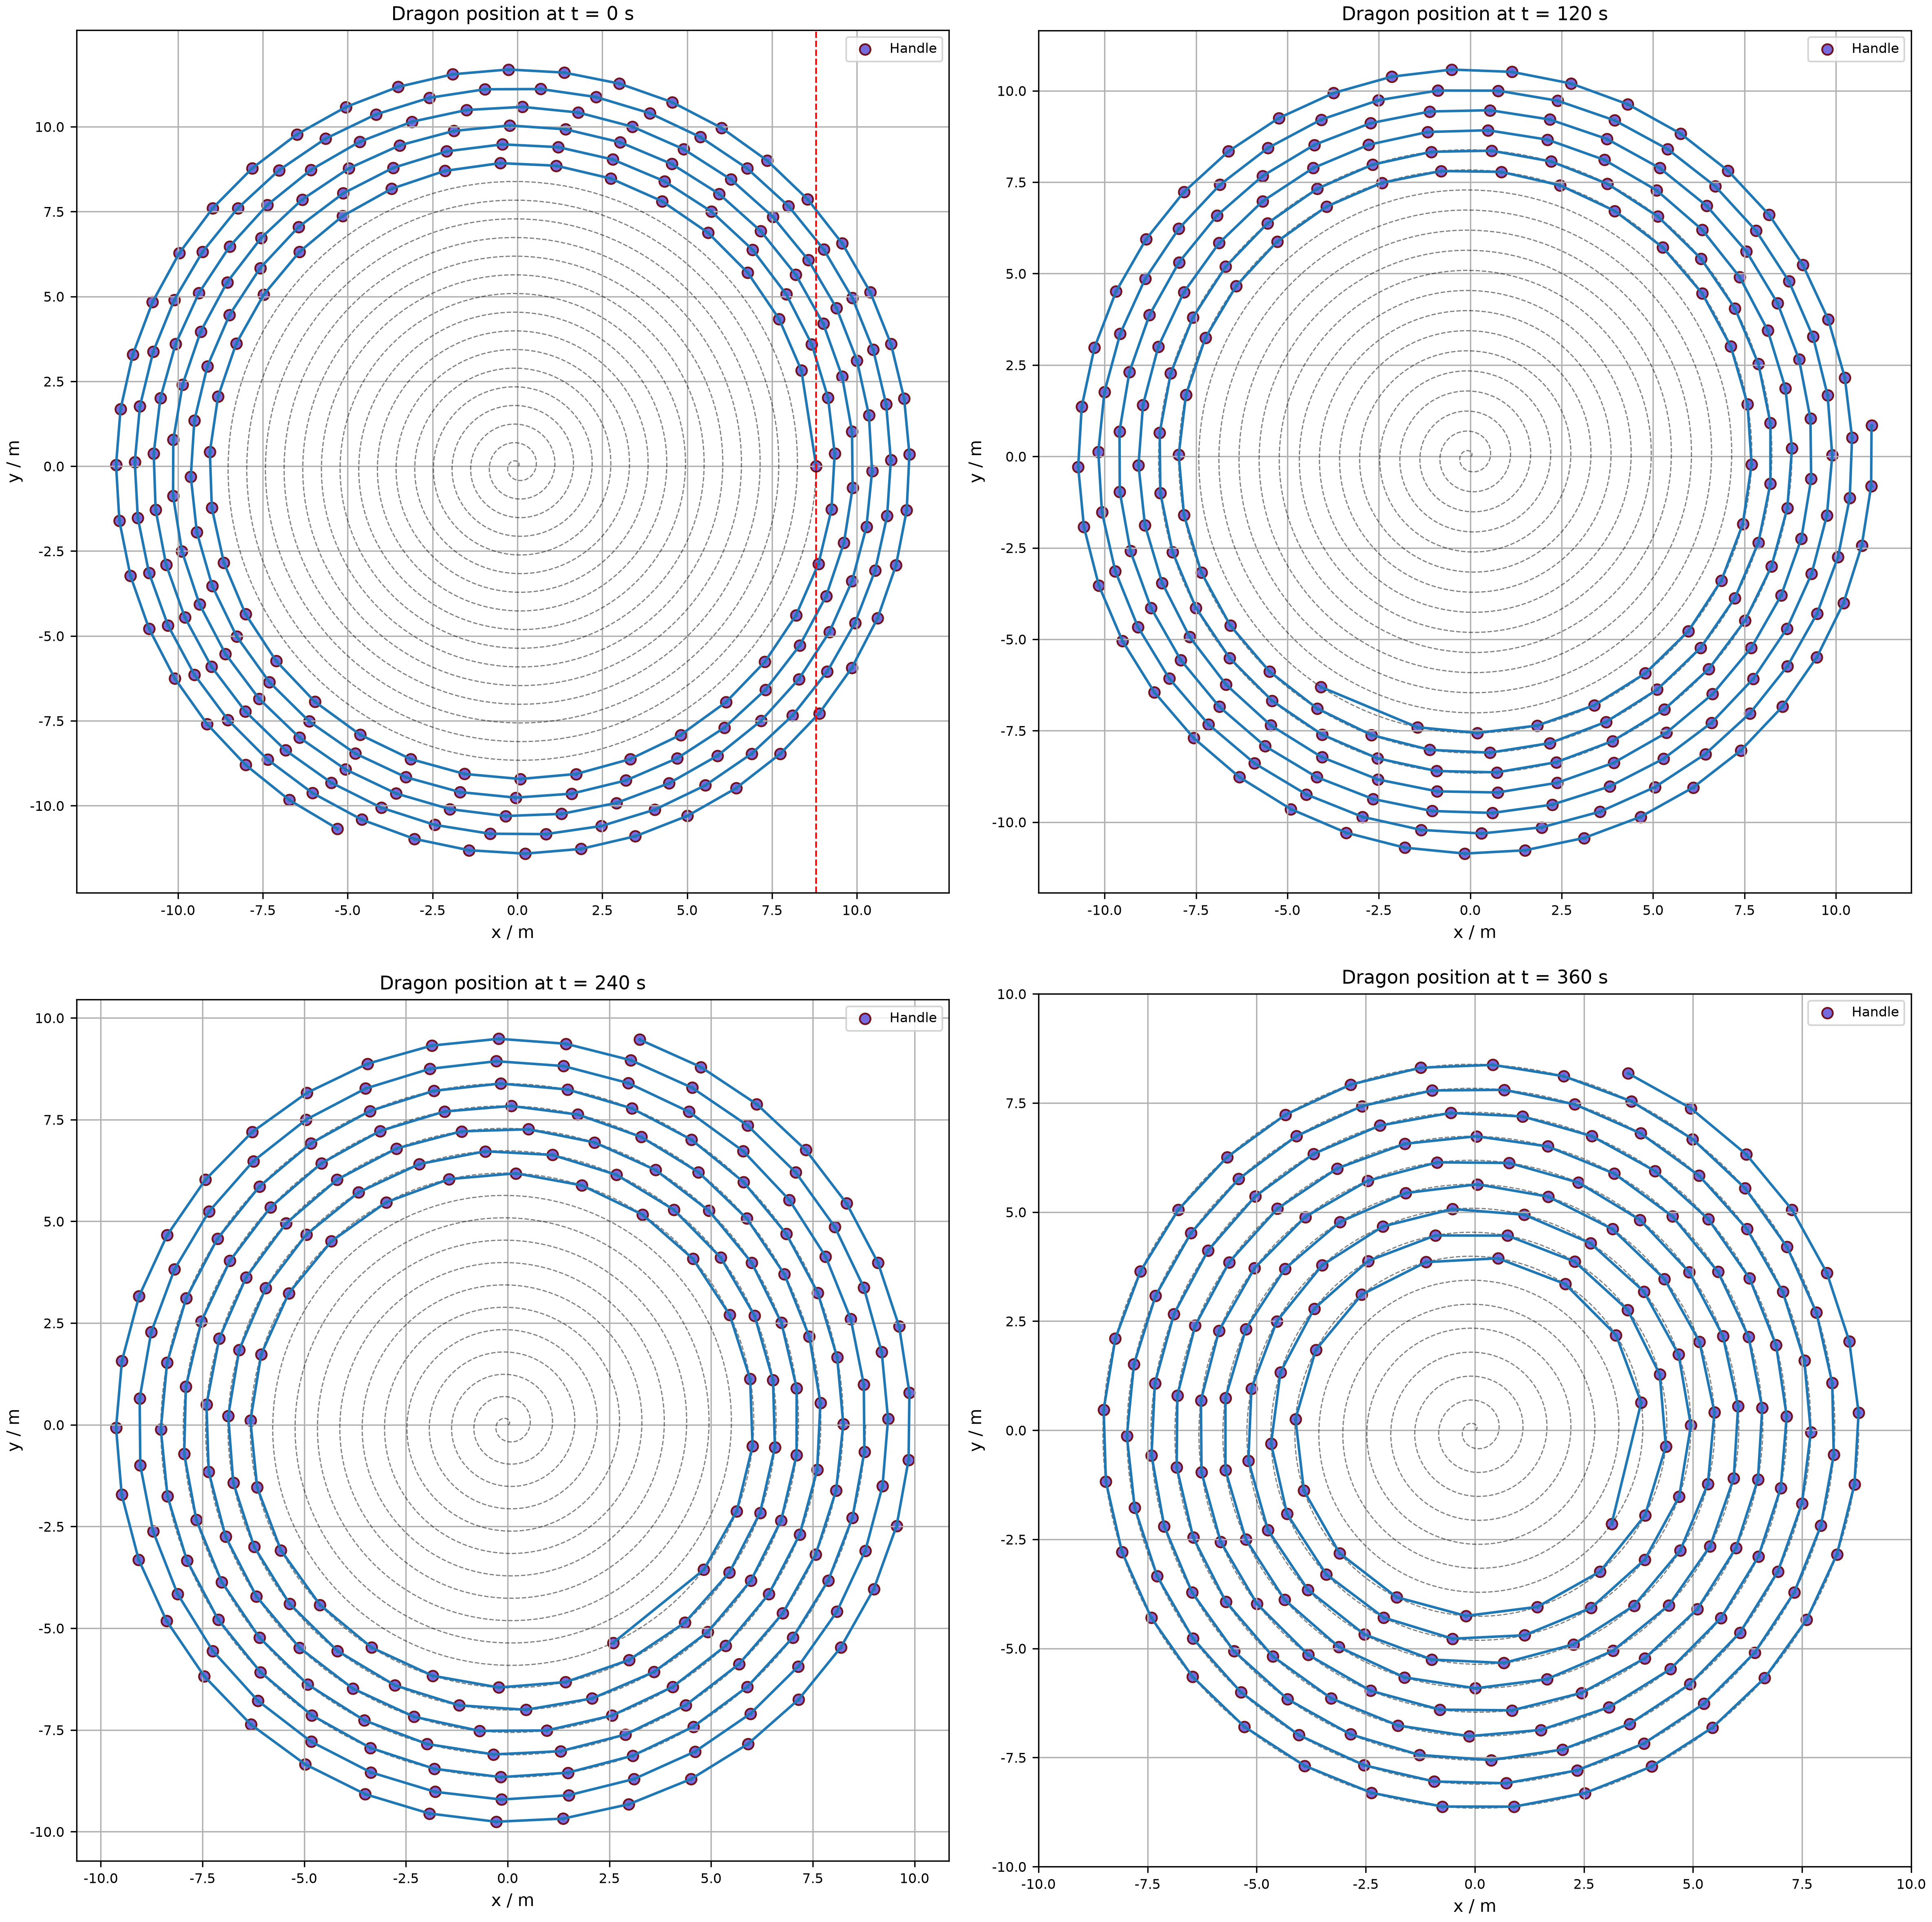
\includegraphics[width=\columnwidth]{images/螺线图 四张.png}
    \caption{板凳龙位置示意图}
    \label{fig:second}
\end{figure}

\subsection{其余把手位置求解}
对于后续其余所有把手的位置，我们仍可以采用二分检验的思想进行求解。为了充分利用几何位置关系，并减轻计算量，我们在极坐标系中的求解过程引入余弦定理进行相邻把手距离的求解。

对于任意一个把手位置：
\begin{equation}
r_i = b\theta_i
\end{equation}
设第$i$个把手和下一个相邻的把手位置的极角差值为$\Delta\theta_i$，则由距离约束：
\begin{equation}
r_{i+1} = b(\theta_i - \Delta\theta_i)
\end{equation}
根据余弦定理：
\begin{equation}
f_i(\Delta\theta_i) = r_i^2 + r_{i+1}^2 - 2r_ir_{i+1}\cos\Delta\theta_i - d_i^2 = 0
\end{equation}
这实际上是得到关于 $\Delta\theta_i$的一个一元非线性方程。
值得注意的是，这里的$d_i$并非固定值。龙头处$d_i$的值为$286$,其余情况均为$165$。

因此，在已知第 $i$个把手参数 $\theta_i$ 的情况下，只需求解上述方程即可得到 $\Delta\theta_i$，进而计算第 $i+1$ 个把手的位置。
值得注意的是，从板凳龙运动过程来看，上述方程并非任意数学根均满足实际要求，第$i+1$个把手应当：

1. 位于当前把手的盘入方向；

2. 与当前把手保持固定距离 $d_i$；

3. 在螺线上与当前把手相邻。

因此我们选取满足约束条件的最小正根作为相邻把手对应的参数间隔
\begin{equation}
\Delta\theta_i = \min\{\Delta\theta > 0 : f_i(\Delta\theta) = 0\}
\end{equation}
方程(16) 难以直接求得解析解，因此采用与 $5.2$ 节相同的二分法进行数值求根，计算精度及终止条件保持一致。
由于当
\begin{equation}
\Delta\theta = 0
\end{equation}
时相邻两个把手重合，有
\begin{equation}
f_i(0) = -d_i^2 < 0.
\end{equation}

随后从 $\Delta\theta = 0$ 开始向右搜索，确定使
\begin{equation}
f_i(\Delta\theta_R) > 0
\end{equation}
的第一个位置，从而得到满足
\begin{equation}
f_i(0)f_i(\Delta\theta_R) < 0
\end{equation}
的初始求根区间
\begin{equation}
[0,\,\Delta\theta_R].
\end{equation}

在此基础上，按照 5.2 节所述二分法不断缩小区间，最终得到
\begin{equation}
\Delta\theta_i \approx \frac{\Delta\theta_L + \Delta\theta_R}{2}.
\end{equation}

再由螺线参数方程得到其平面坐标：
\begin{equation}
\begin{cases}
x_{i+1} = b\theta_{i+1}\cos\theta_{i+1},\\[6pt]
y_{i+1} = b\theta_{i+1}\sin\theta_{i+1}.
\end{cases}
\end{equation}

将 $\theta_{i+1}$ 作为下一次递推的已知量，重复上述过程，即可依次得到
\begin{equation}
\theta_1 \rightarrow \theta_2 \rightarrow \cdots \rightarrow \theta_N
\end{equation}
从而确定该时刻舞龙队所有把手的位置。

% ==================== 表1：位置数据 ====================
\begin{table}[htbp]
    \centering
    \small  % 缩小字体以适应页面宽度
    \caption{各部位在不同时间点的位置坐标}
    \label{tab:position}
    \begin{tabular}{l|r|r|r|r|r|r}
        \hline
        时间点 & 0 s & 60 s & 120 s & 180 s & 240 s & 300 s \\
        \hline
        龙头 x (m)  & 8.800000  & 5.799209  & -4.084887 & -2.963609 & 2.594494  & 4.420274 \\
        龙头 y (m)  & 0.000000  & -5.771092 & -6.304479 & 6.094780  & -5.356743 & 2.320429 \\
        第1节龙身 x (m) & 8.363824  & 7.456758  & -1.445473 & -5.237118 & 4.821221  & 2.459489 \\
        第1节龙身 y (m) & 2.826544  & -3.440399 & -7.405883 & 4.359627  & -3.561949 & 4.402476 \\
        第51节龙身 x (m) & -9.518732 & -8.686317 & -5.543150 & 2.890455  & 5.980011  & -6.301346 \\
        第51节龙身 y (m) & 1.341137  & 2.540108  & 6.377946  & 7.249289  & -3.827758 & 0.465829 \\
        第101节龙身 x (m) & 2.913983  & 5.687116  & 5.361939  & 1.898794  & -4.917371 & -6.237722 \\
        第101节龙身 y (m) & -9.918311 & -8.001384 & -7.557638 & -8.471614 & -6.379874 & 3.936008 \\
        第151节龙身 x (m) & 10.861726 & 6.682311  & 2.388757  & 1.005154  & 2.965378  & 7.040740 \\
        第151节龙身 y (m) & 1.828753  & 8.134544  & 9.727411  & 9.424751  & 8.399721  & 4.393013 \\
        第201节龙身 x (m) & 4.555102  & -6.619664 & -10.627211 & -9.287720 & -7.457151 & -7.458662 \\
        第201节龙身 y (m) & 10.725118 & 9.025570  & 1.359847  & -4.246673 & -6.180726 & -5.263384 \\
        龙尾（后） x (m)  & -5.305444 & 7.364557  & 10.974348 & 7.383896  & 3.241051  & 1.785033 \\
        龙尾（后） y (m)  & -10.676584 & -8.797992 & 0.843473  & 7.492370  & 9.469336  & 9.301164 \\
        \hline
    \end{tabular}
\end{table}



\subsection{速度模型}

设第 $i$ 个把手的位置为
\begin{equation}
    \mathbf{r}_i=\mathbf{r}(\theta_i),
\end{equation}
相邻把手间的刚性连接长度为 $L_i$，则位置约束为
\begin{equation}
    \|\mathbf{r}_{i+1}-\mathbf{r}_i\|^2=L_i^2.
\end{equation}

对其关于时间求导，由于刚性连接长度始终不变，得到：
\begin{equation}
    (\mathbf{r}_{i+1}-\mathbf{r}_i)
    \cdot
    (\mathbf{v}_{i+1}-\mathbf{v}_i)=0.
\end{equation}

又由链式法则，
\begin{equation}
\mathbf{v}_i = \frac{d\mathbf{r}_i}{dt} = \mathbf{r}'(\theta_i)\dot\theta_i.
\end{equation}

令
\begin{equation}
    \mathbf{d}_i=\mathbf{r}_{i+1}-\mathbf{r}_i,
    \qquad
    \mathbf{T}_i=\mathbf{r}'(\theta_i),
\end{equation}
则相邻把手的角速度满足
\begin{equation}
    \dot{\theta}_{i+1}
    =
    \frac{\mathbf{d}_i\cdot\mathbf{T}_i}
    {\mathbf{d}_i\cdot\mathbf{T}_{i+1}}
    \dot{\theta}_i.
\end{equation}

龙头速度 $v_{\mathrm{head}}$ 已知，因此
\begin{equation}
    \dot{\theta}_1
    =
    -\frac{v_{\mathrm{head}}}
    {\|\mathbf{T}_1\|}.
\end{equation}

对于阿基米德螺线 $r=a+b\theta$，有
\begin{equation}
    \mathbf{T}(\theta)
    =
    \begin{pmatrix}
        b\cos\theta-r\sin\theta\\
        b\sin\theta+r\cos\theta
    \end{pmatrix},
    \qquad
    \|\mathbf{T}(\theta)\|=\sqrt{r^2+b^2}.
\end{equation}

因此
\begin{equation}
    \dot{\theta}_1
    =
    -\frac{v_{\mathrm{head}}}
    {\sqrt{r_1^2+b^2}}.
\end{equation}

最终其线速度为
\begin{equation}
    v_i
    =
    \sqrt{r_i^2+b^2}\,|\dot{\theta}_i|.
\end{equation}
由此逐节递推得到所有把手的角速度。

% ==================== 表2：速度数据 ====================
\begin{table}[htbp]
    \centering
    \small
    \caption{各部位在不同时间点的速度}
    \label{tab:speed}
    \begin{tabular}{l|r|r|r|r|r|r}
        \hline
        时间点 & 0 s & 60 s & 120 s & 180 s & 240 s & 300 s \\
        \hline
        龙头 (m/s)       & 1.000000 & 1.000000 & 1.000000 & 1.000000 & 1.000000 & 1.000000 \\
        第1节龙身 (m/s)  & 0.999971 & 0.999961 & 0.999945 & 0.999917 & 0.999859 & 0.999709 \\
        第51节龙身 (m/s) & 0.999742 & 0.999662 & 0.999538 & 0.999331 & 0.998941 & 0.998065 \\
        第101节龙身 (m/s)& 0.999575 & 0.999453 & 0.999269 & 0.998971 & 0.998435 & 0.997302 \\
        第151节龙身 (m/s)& 0.999448 & 0.999299 & 0.999078 & 0.998727 & 0.998115 & 0.996861 \\
        第201节龙身 (m/s)& 0.999348 & 0.999180 & 0.998935 & 0.998551 & 0.997894 & 0.996574 \\
        龙尾（后） (m/s) & 0.999311 & 0.999136 & 0.998883 & 0.998489 & 0.997816 & 0.996478 \\
        \hline
    \end{tabular}
\end{table}

        % 问题1
% ============================================================
% 第5章 问题2 模型建立与求解
% ============================================================

\section{模型建立与求解——问题2}

\subsection{矩形模型构建}
设第 $i$ 节板凳的两个把手中心分别为
\begin{equation}
P_i = (x_i, y_i), \qquad P_{i+1} = (x_{i+1}, y_{i+1}).
\end{equation}

定义板凳中心为
\begin{equation}
C_i = \frac{P_i + P_{i+1}}{2}.
\end{equation}

由两个把手确定板凳中心线方向，定义单位方向向量：
\begin{equation}
\mathbf{e}_i = \frac{P_{i+1} - P_i}{\|P_{i+1} - P_i\|}.
\end{equation}

其法向单位向量为：
\begin{equation}
\mathbf{n}_i = (-e_{iy}, e_{ix}).
\end{equation}

因此，第 $i$ 节板凳可以表示为：

以 $C_i$ 为中心、$\mathbf{e}_i$ 为纵向方向、长度为 $L_i$、宽度为 $w = 0.30\,\mathrm{m}$ 的矩形。

其中
\begin{equation}
L_i =
\begin{cases}
3.41, & i=1, \\[4pt]
2.20, & 2 \le i \le 222.
\end{cases}
\end{equation}

龙尾同样按照实际板长进行处理。
相邻把手距离明确：
\begin{equation*}
d_s = L_s - 2a = 2.20 - 2(0.275) = 1.65\,\mathrm{m}.
\end{equation*}

对于龙头：

\begin{equation*}
L_h = 3.41\,\mathrm{m},
\end{equation*}
\begin{equation*}
d_h = L_h - 2a = 3.41 - 2(0.275) = 2.86\,\mathrm{m}.
\end{equation*}




\subsection{分层碰撞检测}
对于全部$223$节板凳而言，全部直接进行逐一碰撞检测会十分复杂。因此，为了减少计算量和代码复杂度，我们引入分层碰撞检测的方法。

具体而言，我们按照顺序采用：

1. 角度筛选；

2. 圆距离筛选；

3. SAT精检。

\textbf{对于角度筛选}

由于舞龙队沿等距螺线向圆心方向盘入，相邻板凳的极角依次减小。

对于第 \(i\) 节板凳和其后第 \(j\) 节板凳，定义极角差为
\begin{equation*}
\Delta\theta_{ij} = \theta_i - \theta_j > 0.
\end{equation*}

由阿基米德螺线方程
\begin{equation*}
r = b\theta
\end{equation*}

可得两把手的径向距离差为
\begin{equation*}
|r_i - r_j| = b\Delta\theta_{ij}.
\end{equation*}

当
\begin{equation*}
\Delta\theta_{ij} > 3\pi
\end{equation*}

时，有
\begin{equation*}
|r_i - r_j| > 3\pi b = \frac{3p}{2} = 0.825\,\text{m}.
\end{equation*}

因此，随着极角差增大，两板凳在螺线上的空间间隔迅速增大。基于舞龙队的螺线排列结构，本文首先将
\begin{equation*}
0 < \Delta\theta_{ij} \leq 3\pi
\end{equation*}

范围内的板凳作为潜在碰撞对象，对超出该范围的板凳对进行预筛除，以减少后续碰撞检测的计算量。

\textbf{对于圆距离筛选}

为进一步降低矩形精确碰撞检测的计算量，将每节板凳矩形用其外接圆进行包络。

设第 \(i\) 节板凳的中心为 \(C_i\)，长度为 \(L_i\)，宽度为 \(w\)，则其外接圆半径为
\begin{equation*}
R_i = \frac{1}{2}\sqrt{L_i^2 + w^2}.
\end{equation*}

由于板凳矩形完全包含于其外接圆内，因此若两节板凳发生碰撞，则其外接圆必然相交。故由逆否命题可得：
\begin{equation*}
\|C_i - C_j\| > R_i + R_j \Rightarrow \text{板凳 } i, j \text{ 不发生碰撞.}
\end{equation*}

因此，在进行矩形精确碰撞检测前，首先计算两板凳中心之间的距离。若满足上述条件，则直接判定两板凳不存在碰撞，无需进一步进行分离轴定理检测；只有当：
\begin{equation*}
\|C_i - C_j\| \leq R_i + R_j
\end{equation*}

时，才将该板凳对纳入后续的矩形精确碰撞判定。

\subsection{基于 SAT 的精确碰撞判定}

由于相邻板凳本身通过把手连接，因此本文主要判断非相邻板凳之间是否发生碰撞，即当：

\begin{equation*}
|i-j| \ge 2.
\end{equation*}

对于任意两节非相邻板凳 $i,j$，采用分离轴定理（Separating Axis Theorem，SAT）进行矩形相交判定。下面先引入分离轴定理。

分离轴（SAT）定理：对于两个凸矩形，如果存在一条直线方向，使得两个矩形在该方向上的投影区间互不重叠，则两矩形不发生碰撞。

特别地：对于两个矩形，只需考察它们自身的边方向及其法向方向。因此选取以下四个候选方向：
\begin{equation*}
u \in \{ e_i, n_i, e_j, n_j \}.
\end{equation*}


设矩形 \(i\) 的中心为 \(C_i\)，长度为 \(L_i\)，宽度为 \(w\)。

在任意单位方向 \(\mathbf{u}\) 上，其投影半径为：
\begin{equation*}
R_i(\mathbf{u}) = \frac{L_i}{2}|\mathbf{e}_i \cdot \mathbf{u}| + \frac{w}{2}|\mathbf{n}_i \cdot \mathbf{u}|.
\end{equation*}

因此矩形 \(i\) 在 \(\mathbf{u}\) 方向上的投影区间为：
\begin{equation*}
I_i(\mathbf{u}) = [C_i \cdot \mathbf{u} - R_i(\mathbf{u}), C_i \cdot \mathbf{u} + R_i(\mathbf{u})].
\end{equation*}

矩形 \(j\) 同理。

两个矩形在方向 \(\mathbf{u}\) 上发生投影分离，当且仅当：
\begin{equation*}
|(C_i - C_j) \cdot \mathbf{u}| > R_i(\mathbf{u}) + R_j(\mathbf{u}).
\end{equation*}

若对于四个候选方向中的任意一个方向均满足上述不等式，则两个矩形存在分离轴，因此：
板凳 \(i,j\) 不发生碰撞。

反之，如果四个方向均不存在投影分离，即：
\begin{equation*}
|(C_i - C_j) \cdot \mathbf{u}| \leq R_i(\mathbf{u}) + R_j(\mathbf{u}), \quad \forall \mathbf{u} \in \{\mathbf{e}_i, \mathbf{n}_i, \mathbf{e}_j, \mathbf{n}_j\}.
\end{equation*}

则认为两节板凳发生碰撞。

\subsection{首次碰撞时刻的确定}
我们首先定义碰撞状态函数
\begin{equation*}
C(t) = \begin{cases} 0, & \text{时刻 } t \text{ 无板凳碰撞}, \\ 1, & \text{时刻 } t \text{ 存在板凳碰撞}. \end{cases}
\end{equation*}

首次碰撞时刻定义为
\begin{equation*}
t^* = \inf\{t : C(t) = 1\}.
\end{equation*}

首先以一定时间步长对盘入过程进行粗搜索，并在各时刻依次进行“极角范围粗筛—外接圆粗筛—SAT精确判定”，确定满足
\begin{equation*}
C(t_k) = 0, \quad C(t_{k+1}) = 1
\end{equation*}

的时间区间，即
\begin{equation*}
t^* \in [t_k, t_{k+1}].
\end{equation*}

随后沿用问题一中的二分法，在该区间内取
\begin{equation*}
t_m = \frac{t_L + t_R}{2},
\end{equation*}

根据碰撞状态不断缩小搜索区间，直至
\begin{equation*}
|t_R - t_L| < \varepsilon_t.
\end{equation*}

最终取
\begin{equation*}
t^* = \frac{t_L + t_R}{2}
\end{equation*}

作为板凳龙首次发生碰撞的临界时刻。

经计算，板凳龙首次发生碰撞的时间为412.47s。
\begin{figure}[htbp]      
    \centering              % 图片居中
    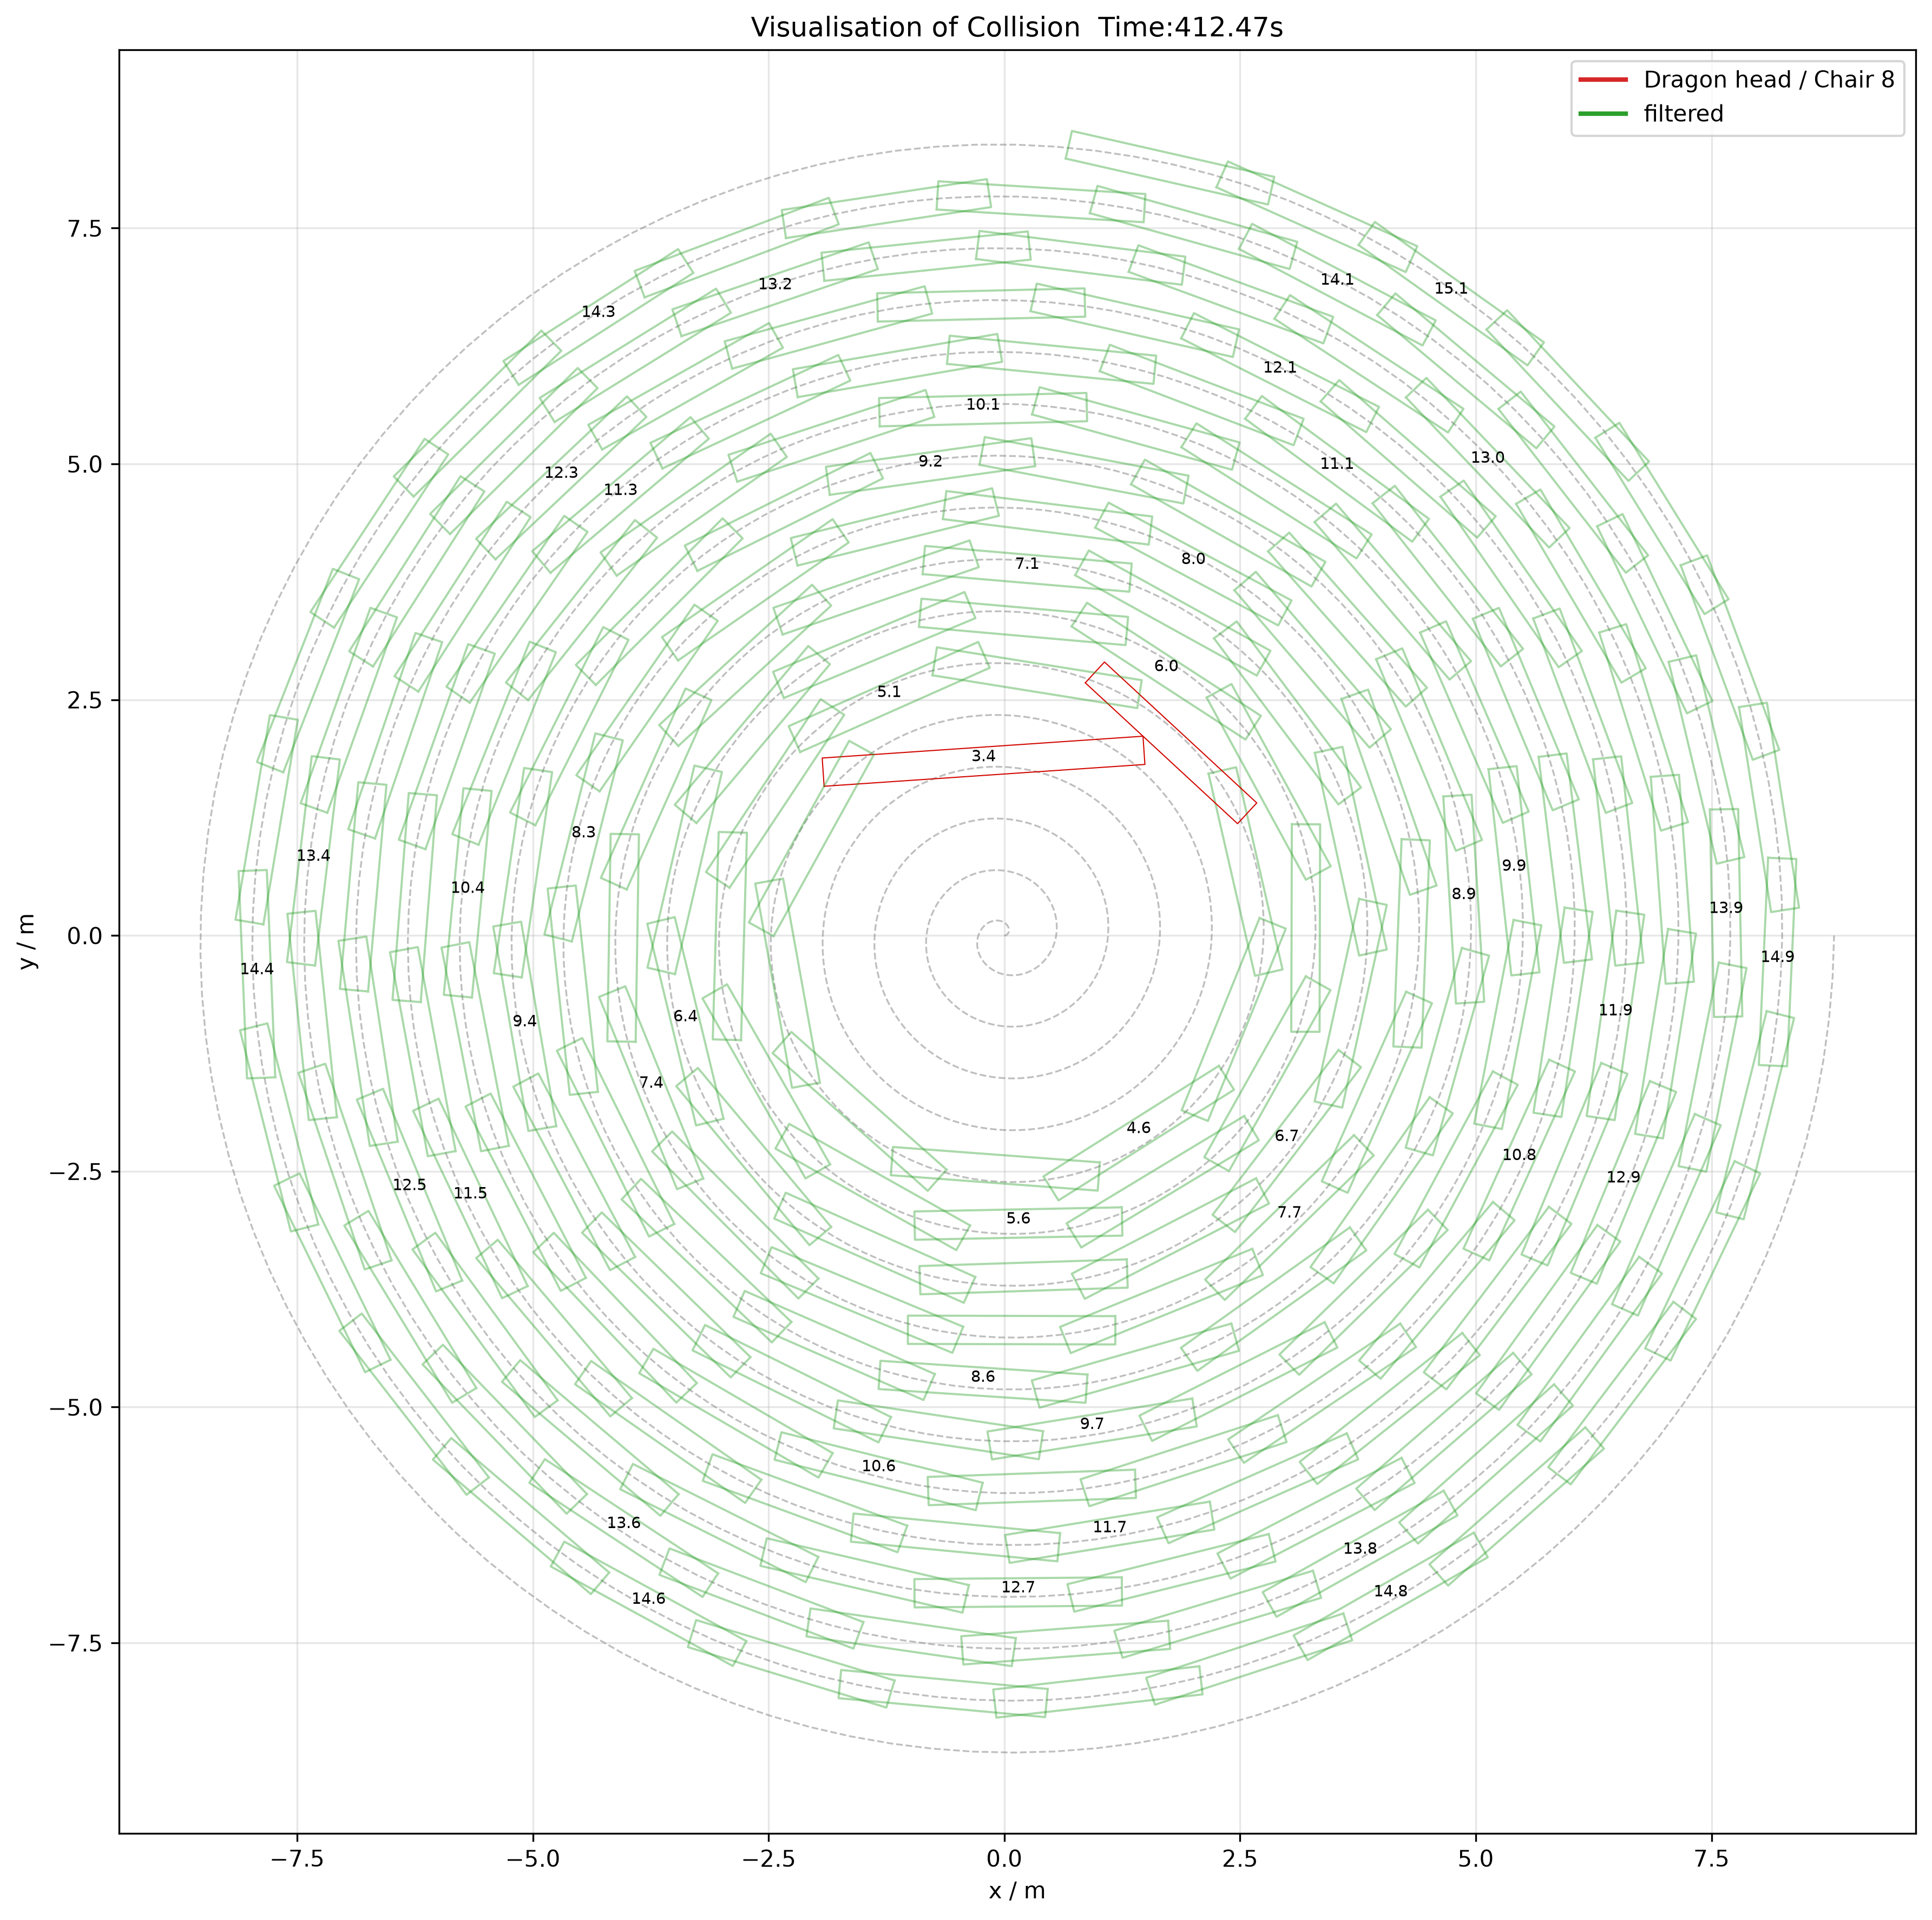
\includegraphics[width=0.8\textwidth]{images/碰撞图 412.47.png} % 插入图片
    \caption{碰撞时刻示意图} % 图片标题
    \label{fig:third}     % 标签，用于引用
\end{figure}



\subsection{各把手的位置和速度的求解}
确定首次碰撞的临界时刻 \(t^*\) 后，利用问题一中的把手位置递推模型求得各把手极角 \(\theta_i(t^*)\)。将其代入阿基米德螺线参数方程，可得各把手位置
\begin{equation*}
P_i(t^*) = (b\theta_i(t^*)\cos\theta_i(t^*), b\theta_i(t^*)\sin\theta_i(t^*)).
\end{equation*}

对位置方程关于时间求导，得到
\begin{equation*}
\dot{x}_i = b(\cos\theta_i - \theta_i\sin\theta_i)\dot{\theta}_i,
\end{equation*}
\begin{equation*}
\dot{y}_i = b(\sin\theta_i + \theta_i\cos\theta_i)\dot{\theta}_i.
\end{equation*}

又由螺线弧长关系
\begin{equation*}
\frac{ds}{d\theta_i} = b\sqrt{1+\theta_i^2}, \quad \frac{ds}{dt} = v,
\end{equation*}

可得
\begin{equation*}
\dot{\theta}_i = \frac{v}{b\sqrt{1+\theta_i^2}}.
\end{equation*}

因此各把手速度大小为
\begin{equation*}
v_i = \sqrt{\dot{x}_i^2 + \dot{y}_i^2} = v.
\end{equation*}


        % 问题2
% ============================================================
% 第6章 问题3 模型建立与求解
% ============================================================

\section{模型建立与求解——问题3}

\subsection{多光束干涉模型}
引入 Airy 公式：
\begin{equation}
    r_{\text{eff}} = \frac{r_{01} + r_{12}e^{i\delta}}{1 + r_{01}r_{12}e^{i\delta}}
\end{equation}
定义多光束效应显著性指标：
\begin{equation}
    G = |r_{01}r_{12}| \exp\left(-\frac{4\pi \kappa_1 d \cos\theta_1}{\lambda}\right)
\end{equation}

\subsection{数据计算与修正}
分别对硅晶片（附件3、4）和碳化硅（附件1、2）进行计算，比较双光束与多光束模型的差异并修正。        % 问题3
% ============================================================
% 第7章 模型检验及合理性分析
% ============================================================

\section{模型检验及合理性分析}

\subsection{误差来源分析}
推导厚度 $d$ 对极值波数 $\tilde{\nu}$ 的灵敏度：
\begin{equation}
    \frac{\partial d}{\partial \tilde{\nu}_i} = \frac{i}{D^2}\left(A_i + \frac{\tilde{\nu}_i n_i n_i'}{A_i}\right)
\end{equation}

\subsection{统计可靠性}
给出各入射角下的平均值、标准差、置信区间和变异系数（CV）。

\subsection{多光束修正验证}
比较双光束与多光束模型的残差平方和，证明修正效果。      % 模型检验
% ============================================================
% 第8章 模型评价与展望
% ============================================================

\section{模型评价与展望}

\subsection{模型优点}
\begin{itemize}
    \item 物理基础扎实...
    \item 方法互补，相互印证...
\end{itemize}

\subsection{模型缺点}
\begin{itemize}
    \item 参数依赖文献...
    \item 平滑方法较简单...
\end{itemize}

\subsection{未来展望}
引入机器学习、拓展到其他材料等。      % 模型评价与展望

% ---------- 参考文献 ----------
% ============================================================
% 参考文献
% ============================================================

\begin{thebibliography}{99}
\bibitem{ref1} 作者. 文章名. 期刊名，年份，卷(期): 页码.
\bibitem{ref2} 作者. 书名. 出版社，年份.
\bibitem{ref3} 作者. 论文题目. 博士学位论文，学校，年份.
\end{thebibliography}

% ---------- 附录 ----------
% ============================================================
% 附录
% ============================================================

\appendix
\section{支撑材料与代码}

\subsection{数据预处理代码}
\begin{lstlisting}[language=Python, caption=样条插值提取极值点]
import numpy as np
from scipy.interpolate import UnivariateSpline
# 此处放你的代码
\end{lstlisting}

\subsection{附加图表}
此处放不便于放在正文中的大图或长表格。

\end{document}
